\documentclass{report}
\usepackage[utf8]{inputenc}
\usepackage{amsmath,amsthm,amsfonts,amssymb,amscd}
\usepackage[a4paper,hmargin=0.8in,bottom=1.3in]{geometry}
\usepackage{lastpage,enumerate,fancyhdr,mathrsfs,xcolor,graphicx,listings,hyperref,enumitem}
\newcommand*{\algodis}[4]{
    \textbf{#1:} #2\\%name: % key idea
    \textbf{Time:} #3 \\% O(what)
    \textbf{Space:} #4
}
\author{Hardik Rajpal}

\begin{document}
\definecolor{codegreen}{rgb}{0,0.6,0}
\definecolor{codegray}{rgb}{0.5,0.5,0.5}
\definecolor{codepurple}{rgb}{0.58,0,0.82}
\definecolor{backcolour}{rgb}{0.95,0.95,0.92}

\lstdefinestyle{mystyle}{
    backgroundcolor=\color{backcolour},   
    commentstyle=\color{codegreen},
    keywordstyle=\color{magenta},
    numberstyle=\tiny\color{codegray},
    stringstyle=\color{codepurple},
    basicstyle=\ttfamily\footnotesize,
    breakatwhitespace=false,         
    breaklines=true,                 
    captionpos=b,                    
    keepspaces=true,                 
    numbers=left,                    
    numbersep=5pt,                  
    showspaces=false,                
    showstringspaces=false,
    showtabs=false,                  
    tabsize=2
}

\lstset{style=mystyle,language=C++}
\title{Pre-Placement Grind}
\maketitle
\tableofcontents
\pagebreak
\chapter{Misc.}
\section{Misc. Confirmed Optimizations}
\begin{enumerate}
    \item For maps,
\begin{lstlisting}
    auto iter = m.find(k);
    if(iter!=m.end()){return iter->second;}
    //is much faster than:
    if(m.count(k)){return m[k];}
\end{lstlisting}
    \item Replace sets that check for inclusion by bit operations with an integer if the number elements $<$ 32 for ints and 64 for long longs. 
    \item Pass params by reference where possible.
    \item Instead of a reference parameter, consider using a pointer to that variable stored in a class data member.
    \item Replace data types by smaller data types where possible:
        \begin{itemize}
            \item long long by int
            \item int by char
        \end{itemize} 
    \item Replace fixed-length vectors by array$<$type,fixed-length$>$.
    \item Replace maps by vectors if they are indexed by integers within a fixed range. Ex: the alphabet as indices.
    \item That die roll problem optimization. (Needs to be phrased more mathematically.)
    \item Use of suffix arrays + descending order (or its prefix counterpart) to cut of paths in backtracking.
\end{enumerate}
\chapter{Week 1}
\section{Searching Algorithms}
\subsection*{Notes from \href{https://www.geeksforgeeks.org/searching-algorithms/}{GFG}}
These are algorithms to check for the existence of an element or to retrieve it from
a data structure. The retrieval can also involve only returning the position (index)
or a pointer to the element. There are two types:
\begin{enumerate}
    \item Sequential search: check every element based on a pre-determined sequence (ex. linear, alternating, etc.),
    and return the matches.
    \item Interval search: Designed for searching in \textbf{sorted} data structures.
    They involve \textbf{repeatedly} dividing the search space into intervals which
    can be excluded entirely after certain checks (ex. binary search).
\end{enumerate}
Some search algorithms are discussed below:
\begin{enumerate}
    \item \algodis{Linear Search}{Straighforward for-loop iterating over all elements in an array.}
    {O(n)}
    {O(1)}
    \item \algodis{Sentinel Linear Search}{Reduces the number of 
    comparisons by eliminating the need to check if the index is 
    within bounds. This is accomplished by appending the target
    element to the end of the array, and treating its index in the result as ``not found."}
    {O(n)}{O(1)}
    \item \algodis{Binary Search}
    {It's used for sorted arrays. It involves comparing the element
    at the center of the interval (defined initially as the entire array),
    with the target element. One of the halves of the interval is picked
    based on this comparison. The interval shrinks until the target is found
    or an interval of size one is not equal to the element. It can
    be implemented recursively or iteratively, each involving a step
    similar to $m = l + \frac{(r-l)}{2}$ while $l \leq r$}.
    {O(log(n))}
    {O(1)}
    \item \algodis{Meta Binary Search}
    {Seems unimportant but check it \href{https://www.geeksforgeeks.org/meta-binary-search-one-sided-binary-search/}{here}}
    {O(log(n))}{O(1)}
    \item \algodis{K-ary Search}
    {The search space is divided into k intervals in each step and one of them is picked to proceed further
    by comparing the target element to the interval markers.}
    {O(log(n)). The reduction is of a constant term: $log_k2$}
    {O(1)}
    \item \algodis{Jump Search}
    {The sorted array is examined in jumps of the
    optimal size $\sqrt{n}$,until the element being examined is greater than
    the target element. The interval is then shrunk to the previous interval.
    The shurnken interval can be examined linearly or with another jump search.
    }
    {O($2\sqrt{n} = O(\sqrt{n})$), or $O(n^{1/2} + n^{1/4} + n^{1/8}...) = O(\sqrt{n})$}
    {O(1)}
    \item \algodis{Interpolation Search}
    {It improves over binary search only if the data is uniformly 
    distributed. It involves selecting the splitting point of the 
    current search space by comparing the target value to the current lower and upper bounds of the space. Linear interpolation involves the following equations:\\
    $
    slope = (arr[r] - arr[l])/(r-l)
    $\\
    $
    m = l + slope \times (x - arr[l])
    $}
    {O(log(log(n))) on average, O(n) WCS.}
    {O(1)}
    \item \algodis{Exponential or Unbounded (Binary) Search}
    {We examine the search space from the lower end $l$,
    comparing $l+2^k - 1$ with the target element $x$, where $k$
    is the number of comparisons so far, until $x < arr[l+2^k - 1]$.
    Then, we examine the interval bounded by $l+2^{k-1} - 1$ and 
    $l+2^k - 1$, using binary search.}
    {O(log(n)), where n is the length of the array or where the 
    first occurrence of the target element exists in an unbounded 
    array.}
    {O(1)}
    \item \algodis{Fibonacci Search}
    {The array must be sorted. We first find the Fibonacci number $f(m)$ that exceeds the length of the given array. We compare the target element to the element at $arr[f(m-2)]$. We pick an interval based on the outcome.}
    {O(log(n))}
    {O(1)}
\end{enumerate}
\subsection*{Misc}
\begin{itemize}
    \item The preferred formula for evaluating the middle point of
    the interval in binary search is
    $m = l + (r-l)/2$, and not
    $m = (l+r)/2$, as the latter can suffer due to overflow.
    \item Global variables can also be used to maintain a ``best value yet" while searching through a space with binary search. For ex. find the first element $\geq$ x in an array.
    \item Problems where an array can be mapped to a boolean variable and is guarranteed to have either
    \begin{itemize}
        \item F...FT...T or
        \item T...TF...F
    \end{itemize}
    and our aim is to find the boundary between true and false
    values can be translated to a binary search problem, with 
    the target as the point where the variable changes:
    arr[i] != arr[i+1].
    \item Remember the \texttt{break} statement in iterative binary search if the middle point element is equal to the target.
    \item One can also binary search for a target range's starting point, instead of just a target. \href{https://leetcode.com/problems/find-k-closest-elements/}{See this problem.}
    \item In some cases, we might want to keep the current middle point \texttt{m} in the search space,
    here we resort to replacing either one of \texttt{r = m - 1} or \texttt{l = m + 1} by \texttt{ = m}
    and change the loop invariant \texttt{l <= r} to \texttt{l < r}. 
\end{itemize}
\section{Sorting Algorithms}
These algorithms rearrange a given array in ascending order.
Various other orders can be achieved by modifying the comparison operator.
A sorting algorithm is \textbf{stable} if it preserves the relative
order of equal elements.
\subsection*{Merge Sort}
The first part of the algorithm recursively handles halves of the given array.
The second part merges the halves sorted by the first part.
It takes O(nlog(n)) time in the \textbf{all cases}. O(n) space is necessary
for the merging side of affairs. Implemented recursively. It's advantages
include stability, parallelizability and lower time complexity. It's disadvantages
include higher space complexity and not being in-place, and that it's not
always optimal for small datasets. 
\subsection*{Quick Sort}
It involves recursively picking an element (\textbf{the pivot})
from the unsorted array, 
placing it so that all elements less than it are before and all
those greater than it are after. Then calling this function on the sub-arrays
after and before the chosen element.
//TODO pseudo code
\subsection*{The Others}
\begin{enumerate}
    \item \algodis{Selection Sort}
    {The given array is viewed in two parts; sorted and unsorted.
    Every iteration involves \textbf{selecting} the minimal element
    and swapping it with the first element of the unsorted part. Hence,
    the boundary of the sorted part is expanded and that of the unsorted
    part has contracted. All of this happens inplace. It isn't stable.}
    {O($n^2$)}{O(1)}
    \item \algodis{Bubble Sort}
    {This involves repeatedly traversing the array,
    swapping any two \textbf{adjacent} elements if they are
    in the incorrect (descending) order, until we encounter
    a run with no swaps. It is stable. With each iteration,
    the last elements of the array are sorted in ascending order.}
    {O($n^2$)}
    {O(1)}
    \item \algodis{Insertion Sort}
    {It involves iterating over the array once, and in each iteration,
    if the current element is less than its left neighbour, we move it
    leftwards until its left neighbour is lower than it. It is in-place
    and stable.}
    {O($n^2$)}{O(1)}
    % \item \algodis{Radix/Counting Sort}
    % {}{}{}
\end{enumerate}
\chapter{Week 2}
See the other notes.pdf
\chapter{Week 3}
\section{Complete Search}
\subsection*{Subset Processing}
We use the function below with 0. (n = size of given set.)
\begin{lstlisting}[language=C++,caption=Subset Generation]
void search(int k) {
    if (k == n) {
        // process subset
        subsets.push_back(subset);
    }
    else{
        search(k+1);
        subset.push_back(k);
        search(k+1);
        subset.pop_back();
    }
}
\end{lstlisting}
\begin{lstlisting}[language=C++]
for (int b = 0; b < (1<<n); b++) {
    //b runs from 00..00 to 11...11
    vector<int> subset;
    for (int i = 0; i < n; i++) {
        if (b&(1<<i)){
            subset.push_back(i)
        };
    }
}
\end{lstlisting}
\subsection*{Permutation Generation}
TODO: write up permutation ideas.
TODO: selection of subsets satisfying a property.
\subsection*{Backtracking En General}
If the dimensions of inputs are smaller than usual, backtracking is an option.
As with other algorithms, you want to maximize this as much as possible. Optimizations
are possible by:
\begin{enumerate}
    \item Transforming the inputs so as to reduce the search space.\\
    Example: If you are searching for a subset whose sum is a given target,
    Searching the space of frequency map is better than searching subsets in the
    untransformed set, at least when duplicates are abundant.
    \item Cutting off fruitless search paths as soon as possible. (Pruning the search tree.)
    \item Specifying "min" requirements before taking a path, and equivalently, specifying "max" allowed values in a path to be explored further.
    \item Optimizing the data structures used to record the current state and restrictions. Particularly,
    \begin{itemize}
        \item Using vectors instead of maps where possible.
        \item Using bitmap \texttt{int}s when only inclusion is to be checked.
    \end{itemize}
    \item Instead of using min/max to bring index values within range, which will likely incur repeated
    searches at the boundary, use an if block to disregard paths associated with values
    that exceed the bounds.
    \item A modification of the needle may speed up the search. For example, the search for a word
    may be sped up by searching for its reversed word if the end letter is less frequent than the letter at
    the start.
    
\end{enumerate}
The abstract code for backtracking looks like ths:
\begin{lstlisting}[language=C++]
    //declare global/class member variables.
    void search(int p){
        //p signifies path/position being inspected
        //in the search space.
        if(searchTerminalConditions()){
            if(globalVarSolutionValid){
                //update collection of solutions.
            }
        }
        else{
            for(possible path of exploration){
                //(1)update global vars so as to take this path.
                search(p+1);
                //(2)undo the updates made to global variables.
                //(not necessary if (1) overrides/uses previous updates.)
            }
            //undo any leftover changes made to global variables.
        }
    }
\end{lstlisting}
\textbf{Pruning:} A way of adding intelligence to the backtracking algorithm and
reducing the time spent in fruitless paths. Additionally, we can leverage symmetries
of the search space to check only a fraction of the entire possible solution set. Clearly,
optimizations at the start of the search tree save a lot more time than those at the end.
\subsection*{Meet in the Middle}
Another name for \textbf{Divide and Conquer}. It refers to splitting the search space up
into two halves and combining the results of the two halves. It works if there is an
efficient way to combine the results. Even 1 level of splitting (and extracting solutions
from the halves using brute force) can have worthwhile optimizations: O($2^n$) $\implies$ O($2^{n/2}$).

\chapter{Week 4}
\section{Greedy Algorithms}
\subsection*{\href{https://leetcode.com/discuss/general-discussion/1061059/ABCs-of-Greedy}{Reading Notes}}
Greedy Solutions focus on looking at the problem in smaller steps, and at each step
we select the option that offers the most obvious and immediate benefit. It's sort
of like assuming there's only one maximum point in the search space, and hence,
we just move in the direction with the most inclination. Some popular greedy 
algorithms are:
\begin{itemize}
    \item Dijkstra's shortest path.
    \item Kruskal's minimum spanning tree.
    \item Prim's minimum spanning tree.
    \item Huffman encoding.
\end{itemize}
With greedy algorithms, we often have to repeatedly pick
the minimal element from a collection; hence using a \texttt{priority\_queue}
or a \texttt{multiset} is often helpful.
\subsection{Union Find}
The data structure can also show up in greedy algorithms.
Given below is the most optimized implementation of \texttt{find} and \texttt{combine}.
\begin{lstlisting}[language=C++]
vector<T> items;//given vector of items.
vector<int> root;//representative roots of trees array.
vector<int> rank;//for combine optimization.
int find(int u){
    if(root[u]==u){return u;}
    //instead of return find(root[u]), do:
    root[u] = find(root[u]);//path compression
    return root[u];
}
void combine(int u, int v){
    int ru, rv;
    ru = find(u);rv = find(v);
    if(ru!=rv){
        //u, v in different trees.
        if(rank[ru] < rank[rv]){
            root[ru] = rv;
            rank[rv] += rank[ru];
            //combined tree has least possible height.
        }
        else{
            root[rv] = ru;
            rank[ru] += rank[rv];
        }
    }
}
\end{lstlisting}
\subsubsection*{Variations of \texttt{root} array}
The usual union-find implementation's root elements satisfy 
\texttt{root[r] == r}. However, we can also use negative numbers
at \texttt{root[r]} (which can't be the index of any parent),
and check for \texttt{root[r] < 0} when searching for the root. Such
a setup allows for recording information in the domain of negative
numbers at the root, say, the size of the tree, but negated. The
combine function then simply sets the combined tree's
root value to the confluence of values at \texttt{rv} and
\texttt{ru}.
\subsubsection*{Kruskal's MST Algorithm}
\begin{enumerate}
    \item Have a min-heap of all edges.
    \item Iterate through the heap, merging the trees of the vertices
    of each edge. For each non-trivial merge, update a counter. Additionally, add the edge to the list of edges for the MST or
    its weight to the weight of the MST.
    \item Once the merge counter is at $|V|$ - 1, break.
\end{enumerate}
\subsubsection*{Prim's MST Algorithm}
\begin{enumerate}
    \item Pick a starting vertex. Initialize an empty min-heap of edges. Maintain a count of visited vertices.
    \item Mark current vertex as visited.
    \item Add all edges going out of the current vertex to the heap.
    \item Iterate through the heap until an edge to an unvisited point is found.
    \item Set this point as the current point. Iterate until count of visited vertices = $|V|$.
\end{enumerate}
\subsubsection*{Dijkstra's Shortest Path}
\begin{enumerate}
    \item Pick a starting vertex. Maintain an array of minimum distances to reach any vertex from a visited vertex. For visited vertices, this should be -1.
    \item Update distances of array elements as min(old distance, distance from current point which is INT\_MAX if they are not neighbours). While iterating, record the array element with minimum distance to it. 
    \item Set the recorded element as the current vertex and continue until the current vertex is the target vertex.
\end{enumerate}
Modifications can be made to record the predecessors in the paths
or calculate the weights of the paths.
\begin{lstlisting}[language=C++,caption=Shortest Path]
int distance(vector<int> &pi, vector<int> &pj);
int dijkstras(vector<vector<int>>& ps, int s, int target) {
    int n = ps.size(), res = 0, i = s;
    vector<int> min_d(n, INT_MAX);
    while (i != target) {
        min_d[i] = -1;
        int min_j = i;
        for (int j = 0; j < n; ++j){
            if (min_d[j] != -1) {//visited vertices.
                min_d[j] = min(min_d[j],distance(ps[i],ps[j]));
                min_j = min_d[j] < min_d[min_j] ? j : min_j;
            }
        }
        res += min_d[min_j];
        i = min_j;
    }
    return res;
}
\end{lstlisting}
\begin{lstlisting}[language=C++,caption=Dijkstra's MST]
int distance(vector<int> &pi, vector<int> &pj);
int dijkstras(vector<vector<int>>& ps, int s, int target) {
    int n = ps.size(), res = 0, i = s,connected = 0;
    vector<int> min_d(n, INT_MAX);
    while (connected < n) {
        min_d[i] = -1;
        connected++;
        int min_j = i;
        for (int j = 0; j < n; ++j){
            if (min_d[j] != -1) {//visited vertices.
                min_d[j] = min(min_d[j],distance(ps[i],ps[j]));
                min_j = min_d[j] < min_d[min_j] ? j : min_j;
            }
        }
        res += min_d[min_j];
        i = min_j;
    }
    return res;
}
\end{lstlisting}
\subsubsection*{Stack Based Questions}
These usually involve finding the (lexicographically) minimal
subsequence. We maintain a stack to track the sequence
selected so far. To reverse a stack to get the subsequence, the
most optimal method is:
\begin{lstlisting}[language=C++]
while(s.size()){
    ans.push_back(s.top());
    s.pop();
}
reverse(ans.begin(),ans.end());
\end{lstlisting}
\subsubsection*{Heap+Queue}
Honestly I've only seen one question with this paradigm. However,
it's worth a shot if you realize you have to process numbers
starting always with the largest/smallest element, and have to 
track elements being available/unavailable over time.
I know that's a very vague and oddly specific situation,
but I couldn't just walk by a problem and not make this note.
\\
Additionally, in scheduling problems, consider trying to find
a way to arrange the given tasks, which might result in a
closed form solution.
\subsection{Greedy Matching}
Given two arrays to match elements such that the matching function
can be put into a total order over the elements (ISTG I will word this better,
later), we can sort two arrays and take the first matches offered
by traversing one array, selecting the first matched element with
the element being traversed.
\subsection{Misc Data Structures}
Multiple problems tagged "Greedy" are really just a matter of
organizing the input data in a structure such as a (frequency)
map or a heap. Or we're just sorting the input array.
So, consider this when thinking of approaching 
a question greedily.
\chapter{Week 5}
\section{Dynamic Programming}
A common optimization to look out for when writing the code
for dynamic programming problems, try to ensure that
\begin{enumerate}
    \item The code doesn't compute paths that aren't going to be useful.
    \item The code doesn't recompute any path more than once.
\end{enumerate}
As per \href{https://leetcode.com/problems/house-robber/discuss/156523/From-good-to-great.-How-to-approach-most-of-DP-problems}{this article}, the approach to most dynamic programming problems can be broken
down to:
\begin{enumerate}
    \item Find recursive relation.
    \item Recursive (top-down).
    \item Add Memoization.
    \item Iterative + memoization (bottom-up).
    \item Further optimizations.
    \begin{itemize}
        \item Discarding paths
        \item Reducing space complexity.
    \end{itemize}
\end{enumerate}
\subsection{Common Patterns}
\subsubsection{Min (Max) Path to Reach Target}
\subsubsection{Distinct Ways}
\subsubsection{Merging Intervals}
\subsubsection{DP on Strings}
\subsubsection{Decision Making}
\chapter{OOP (in C++)}
\section{OOPs}
\begin{itemize}
    \item Access-specifiers:
    \begin{enumerate}
        \item private: can only be accessed inside the class.
        \item protected: can be accessed inside the class and inside derived classes.
        \item public: can be accessed everywhere.
    \end{enumerate}
\end{itemize}
\section{Inheritance from \href{https://www.tutorialspoint.com/cplusplus/cpp_inheritance.htm}{TutorialsPoint} and LearnCpp.com}
\begin{lstlisting}[language=C++,caption=Syntax]
    class DerivedClass: access-specifier BaseClass{
        //access-specifier is one on public/private/protected.
    };
\end{lstlisting}
\begin{itemize}
    \item Allows us to define a class in terms of another class.
    \item Derived classes inherit properties of base classes.
    \item Inheritance implements "is-a" relationship. Ex: mammal is-a animal, dog is-a mammal => dog is-a animal also holds.
    \item Derived classes inherit all properties of base classes except:
    \begin{enumerate}
        \item Constructors, destructors and copy constructors.
        \item Overloaded operators.
        \item Friend functions.
    \end{enumerate}
    \item The base classes can be inherited through public, 
    protected or private inheritance, which is specified the 
    access specifier before its name in the declaration of the 
    derived class. The results are:
    \begin{enumerate}
        \item Public: access permissions of public and protected members of the base class are carried forward in the inherited class.
        \item Protected: access permissions of public and protected members of the base class are lowered to protected.
        \item Private: access permissions of public and protected members of the base class are lowered to private.
    \end{enumerate}
\end{itemize}
\subsection{Multiple Inheritance}
\begin{lstlisting}[language=C++,caption=Syntax]
    class DerivedClass: access-specifier baseA, access-specifier baseB ... {
    //access-specifier is one of public/protected/private.
    };
\end{lstlisting}
\begin{itemize}
\item \textbf{Mixins}: a small class that can be inherited from (in combination with other classes) to add properties to the derived class.
\item The constructors of parent base classes are called in the order that they are declared and before the constructor of the derived class.
\item Note that destructors are called in the completely reverse order of constructors. (Think of it as a stack of objects of base classes, with the derived class at the top).
\begin{lstlisting}[language=C++]
class Derived: public Base1, public Base2...
//base1 constructor.
//base2 constructor.
//derived constructor.
...
//derived destructor.
//base 2 destructor.
//base 1 destructor.
\end{lstlisting}
\item If two parent classes contain members with the same signature (name, args), a call to the signature from their common child class' object raises a compilation error. This is resolved using scope resolution operators.
\end{itemize}
\subsubsection{Diamond Problem of Multiple Inheritance}
\begin{itemize}
\item When two parent classes that share a base class are used to derive a child class, the inheritance tree looks like this:
\begin{center}
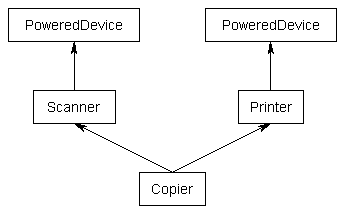
\includegraphics{rsrc/PoweredDevice2.png}
\end{center}
\item Each parent class has its own copy of the base class data members (resulting in redundant copies), and we can't call public members of the base class from the new derived class.
\item The diamond problem refers to our liking for a single instance of the base class in such cases of multiple inheritance, which is different from what happens when we try to implement such a hierarchy.
\item The solution is to use the keyword virtual while declaring the parent classes to identify them as virtual base classes:
\begin{lstlisting}[language=C++]
    class base{};
    class b1: virtual public base{};//
    class b2: virtual public base{};//without virtual in both of them, copies are made.
    class derived: public b1, public b2{};
\end{lstlisting}
\begin{itemize}
    \item Without \texttt{virtual}, each parent class maintains its copy of variables from the base class,\\
    and sizeof(derived) = (sizeof(b1)+size(b2)).
    \item With \texttt{virtual},\\ sizeof(derived) = (sizeof(b1 without b data)+sizeof(b2 without b data) + sizeof(b)+16B)
    \item The 16B are for book keeping. It can also be 8B on some systems.
    \item Note that all parent classes are prefixed with \texttt{virtual} and share ancestors, have a single copy of the ancestor's variables in the derived class.
    \item The book-keeping info grows with 8B for each new parent class. It doesn't grow with the size of the base class (or any class).
\end{itemize}
\item The construction of the base class becomes the responsibility of the derived class:
\begin{lstlisting}
class Copier: public Scanner, public Printer{
public:
Copier():PoweredDevice()/*base class*/, Scanner(), Printer(){
    //Order of constructor defintions run.
    //Base
    //base1
    //base2
    //Derived
}
}
\end{lstlisting}
\item The point above is true because of Printer, Scanner being virtual base classes. The order of constructors holds \textbf{even when single inheritance is done from a virtual base class}.

\item Accessing members of the root class, using an object of a class derived from two non-virtual sibling descendants of the root, leads to compilation errors. To avoid this, either declare the siblings as virtual descendants or use scope resolution operators (of the sibling classes, not the root!).
\end{itemize}
\section{Overloading}
TODO order of usage around operators study.
\begin{itemize}
    \item A single identifier (function name/operator) corresponds to two different implementations, based on the argument list supplied to it.
    \item Overload resolution refers to the compiler's task of selecting the most appropriate implementation when it encounters a call to an overloaded function.
    \item Note: operators can be overloaded outside classes too:
    \begin{lstlisting}[language=C++]
        //As a member function:
        Box operator+(const Box&);
        //Not as a member function:
        Box operator+(const Box&, const Box&);
    \end{lstlisting}
    \item In general, use const and \& for operands to 
    \begin{itemize}
        \item Avoid accidentally modifying them in the operation.
        \item Avoid time spent copying them around.
    \end{itemize}
    \item Most operators can be overloaded:
    \begin{center}
        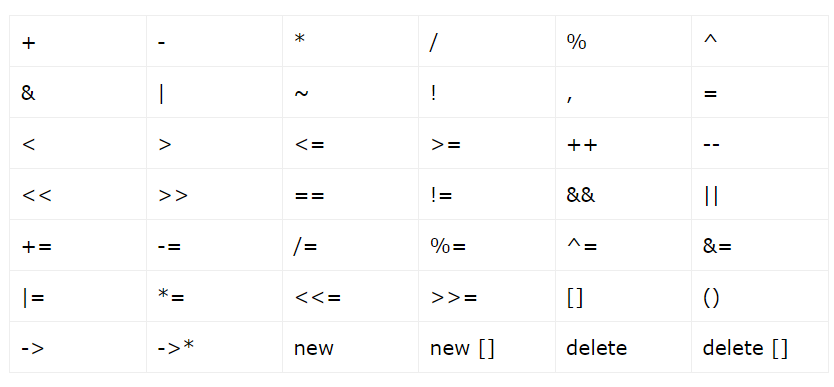
\includegraphics[width=8cm]{rsrc/overloadableops.png}
    \end{center}
    \item Operators that can't be overloaded:
    \begin{enumerate}
        \item ::
        \item .*
        \item .
        \item ?:
    \end{enumerate}
    \item Unary operators include: ++ (post,pre), -- (post,pre), -, ~ and !
\end{itemize}
\subsection{Overloading ++ (and --)}
\begin{lstlisting}[language=C++]
class Digit{
//postfix: a++ : returns an rval.
Digit operator++(int){
    ... return digit;
}
//prefix: ++a : returns an lval. (original variable)
Digit& operator++(){
    ... return *this;
}
}
\end{lstlisting}
\begin{itemize}
\item Both definitions have something unique:
\begin{enumerate}
    \item \& in the prefix definition, to ensure it returns an lvalue.
    \item (int) in the postfix definition is necessary to distinguish it from the prefix definition, as c++ doesn't support return-value-based overloading.
\end{enumerate}
\item Also note that though operator++(int) looks like ++a (prefix), it's actually for a++ (postfix).
\end{itemize}
\section{Polymorphism}
Polymorphism means a call to a member function (after resolution of overloads), can lead to different implementations being called, based on the type of object that invokes the function.
\subsection{Static Linkage}
\begin{lstlisting}[language=C++]
class Shape {
   public:
      int area() {
         cout << "Parent class area :"...
      }
};
class Rectangle: public Shape {
   public:
      int area () { 
         cout << "Rectangle class area :"...
      }
};
class Triangle: public Shape {
   public:
      int area () { 
         cout << "Triangle class area :"... 
      }
};
int main() {
   Shape *shape;
   Rectangle rec(10,7);
   Triangle  tri(10,5);
   shape = &rec;
   shape->area();
   shape = &tri;   
   shape->area();
   //both calls print "Parent class area:..."
   return 0;
}
\end{lstlisting}
Without any prefixes in the functions defined in the derived classes (that are identifiable with functions in the base class),
the compiler assumes that any calls to these functions from an object of type base*/base always needs the implementation from the parent class. This is known as static linkage or static resolution (of the function call) or early binding, as the implementation for the area function is fixed at runtime to that of the base class (for objects of or pointers to the base class).\\
Note that calls from \texttt{rec} or \texttt{tri} would have called their respective functions, not the base class' function.
\subsection{Dynamic Linkage}
Prefixing function identifiers that are shared across derived and base classes with \texttt{virtual}, allows for dynamic linkage, or dynamic resolution or late binding. With the said prefix, the compiler identifies the right implementation to call by the contents of the object or pointer being used to invoke the function. This is polymorphism.
\subsubsection{Pure Virtual Functions}
If a function is always intended to be overridden in the derived classes and there's no meaningful definition in the base class,
we can just declare the function in the base class and set it to zero to avoid compilation errors about no definition being found for
the function in the base class.
\begin{lstlisting}[language=C++]
class Shape{
    //virtual int area();
    //Above line compiles if there are no to area() from any objects of shape/derived classes.
    //In the presence of such calls, even if area() is defined in derived classes and their
    //objects are used to call area() (from the right pointer, or a pointer of type Shape*)
    //compilation errors ensue.
    //However,
    virtual int area()=0;//goes through compilation successfully.
};
\end{lstlisting}
Note:
\begin{itemize}
\item We say a function demonstrates polymorphism if we can use a pointer of the base class
to access functions of different derived classes and have different implementations
being used based on the derived class to which the object belongs. 
\item Without the virtual keyword, even if functions with identical identifiers (name
and arguments considered) are declared in derived and base classes, polymorphism is not
observed. Function calls from pointers of the base class' type call its own implementation,
not that of derived classes. 
\item Once a function is declared as virtual in a class, it demonstrates polymorphism 
across all derived descendant classes, even without the virtual keyword being present 
intermediate classes.
\item The \texttt{final} keyword can be used to throw a compilation error if a function
that we don't want any base classes to override is overridden:
\begin{lstlisting}[language=C++]
class Rectangle:public Shape{
    public:
    int area()final{
        cout<<"Rect Area"<<endl;
        return 0;
    }
};
//Now if a class called square attempts to override area, a compilation error is thrown.
\end{lstlisting}
\item Using the final keyword in a non-virtual function (that was not declared to be virtual in any of the ancestors) throws a compilation error.
\item \textbf{Object Slicing:} When an object of a derived class is assigned to an object (not a pointer) of
a base class, only members inherited from the base class are kept and the others are discarded. Thus,
all functions that may have been overridden are reverted to their definitions in the base class.
\begin{lstlisting}[language=C++]
void printarea(Shape s){
    s.area();
}
void printareaReference(Shape &s){
    s.area();//NO slicing. 
}
Shape s; Rect r;
s = r;//slicing.
Shape &s = r;
printarea(r);//slicing. prints "Shape area..."
printareaReference(r);//No slicing. prints "Rectangle area..."
\end{lstlisting}
In JAVA, and other languages where each non-primitive variable is actually a reference, object
slicing doesn't happen.
\end{itemize}
\section{Data Abstraction and Encapsulation}
The idea is to write classes with a well-defined boundary between:
\begin{enumerate}
\item Implementation: how the class works, the variables and functions it needs for its work.
\item Interface: the function calls and variables accessible to the users of the class.
\end{enumerate}
Data abstraction allows:
\begin{itemize}
\item Implementation of a class to evolve without affecting code that uses it.
\item Prohibiting users from possibly disturbing the state of the objects of the class,
which may affect correctness of its functions. Ex. A user sets the \texttt{top} pointer
inside a stack's implementation to the start of the array, without updating the length,
which is non-zero. This results in a segmentation fault.
\end{itemize}
It is enforced using access specifiers. Data encapsulation is about
bundling all the related data and functions that use it into one class,
keeping as much implementation detail from the user as possible.
\section{Abstract Classes a.k.a C++ Interfaces}
An abstract class is a class with at least one \textbf{pure virtual function}.
Such classes define an interface that all derived classes have to support (have an
implementation of).
\section{Notes from interview questions}
\begin{itemize}
    \item In multilevel inheritance (A->B->C), any function calls from an object of type C are linearly searched for up the hierarchy, and the first implementation is taken.
    \item Pointers of a parent type can hold a child, but child pointers being assigned to parent objects raises compilation errors.
    \item Pointers of a parent type can only access members (variables and functions) declared and declared public in the parent.
    \item When a derived class defines a function with the same name as some function its base class, all functions (even with different signatures) of the base class with the same name become inaccessible to objects.
    \item However, using a pointer of the base type to point to the object of the derived class, both the overridden method and the unoverridden overload of a method with the same name can be accessed.
    \item Or, using a scope resolution operator:
    \begin{lstlisting}[language=C++]
        d.Base::fun(5);//goes through.
        Base &b = d;
        b.fun(5);//goes through.
    \end{lstlisting}
\end{itemize}
\subsubsection{Initializer Lists}
\begin{itemize}
\item Initializer lists of a derived class can't
include members of the base class. They need to be initialized using the contructor of the base class.
\end{itemize}
\subsection{Copy Constructors}
\begin{lstlisting}[language=C++]
class Sample{
    int id;
    Sample(Sample &t)
    {
        id=t.id;
    }
};
//defines what do to do when:
Sample a,b;
a = b;//calls copy constructor of a.
\end{lstlisting}
\begin{itemize}
\item Used to intialize members of a newly created object by copying members of an already existing object.
\item It takes a reference parameter of an object of the same class.
\item This is known as copy initialization, a.k.a. member-wise initialization.
\item If not defined explicitly by the programmer, the compiler 
defines it for us.
\end{itemize}
\subsubsection{Types of Copy Constructors}
\begin{enumerate}
\item Default Copy Constructor: The implementation offered by the compiler which copies the bases and members of an object in the same order that a constructor would intialize the bases and members of the object.
\item User Defined Copy Constructor: needed when an object owns pointers or non-shareable references, such as to a file. A destructor and assignment operator should also ideally be written in this case to assist in transfer/destruction of said references.
\end{enumerate}
A copy constructor is called when:
\begin{itemize}
\item An object of the class is \textbf{returned by value.}
\item An object of the class is \textbf{passed by value} as an argument.
\item An object is constructed based on another object of the same class. Ex: \texttt{Shape s1 = {1,2}; Shape s2(s1) or Shape s2 = s1;}
\item The compiler generates \textbf{a temporary object.}
\end{itemize}
Note that it's not called when a previously declared object is assigned another object. This calls the assignment operator.
\begin{lstlisting}[language=C++]
Shape s1,s2;
s1 = {1,3};
Shape s3(s1);//calls copy constructor.
Shape s4 = s1;//calls copy constructor.
s2 = s1;//calls assignment operator.
\end{lstlisting}
Note that a call to the copy constructor is not guarranteed as
the compiler performs optimizations like \textbf{return value 
optimization} and \textbf{copy elision} to avoid unnecessary 
copies where possible. (TODO)\\
Other points:
\begin{itemize}
\item Use a user-defined copy constructor when the default copy constructor results in a shallow copy (say, if some members are pointers). Deep-copy is only possible in a user-defined constructor.
\item Copy constructors can be made private, and this makes objects of the class non-copyable. It's particularly useful (as a lazy technique to avoid shallow copies) if the class has pointers of dynamically allocated resources. The right way is to write a deep-copy-constructor and make it public.
\item A copy constructor which takes the object argument by value leads to a compilation error, as at runtime it would have lead to an infinite chain of copy constructor calls.
\item Use const in the argument to make sure:
\begin{enumerate}
    \item The source object isn't accidentally modified.
    \item The copy-constructor can be called with temporary objects created by the compiler, which can't be bound to non-const references.
    \begin{lstlisting}[language=C++]
        //if copy constructor doesn't say const Shape &s1,
        Shape s2 = fun();//fun returns s2 by value.
        //the above code throws a compilation error, at the last line.
        //If const is present, it compiles.
    \end{lstlisting}
\end{enumerate} 
\item In default constructors, default constructors of parents are called before those of derived classes, but, in copy constructors, the parent's default constructors (not copy constructors are called), unless the implementation of the derived class' copy constructor specifically calls their copy constructors.
\end{itemize}
\subsubsection{Copy Elision (a.k.a. Copy Omission)} 
The compiler avoids making copies of objects (in pass by value/return by value scenarios) where possible.

\section{From LearnCPP.com}
\subsection{14.4 Const objects}
\begin{lstlisting}[language=C++]
const Date today {2020, 10, 14};//valid.
const Date today = {2020, 10, 14};//valid.
//Note that const objects must be initialized, unless a default
//constructor is defined.
\end{lstlisting}

Objects that are declared with \texttt{const} keyword (as a local variable, or a function argument) impose certain restrictions (that upon violation lead to compiler errors.):
\begin{itemize}
\item Their members variables can't be changed, neither via direct access nor calls to member functions that change them.
\item Additionally, const objects can't call non-const member functions. \texttt{const} before the definition body indicates that the member function doesn't modify the members of the class; it doesn't impose any restrictions on the returned value or aruments.
\begin{lstlisting}[language=C++]
class Date{
    //can't be called by a const object, despite not
    //altering any variables in its definition:
    void print(){
        cout<<"non-const member function.";
    }
    //can be called by const objects:
    void print2() const {
        cout<<"const member function.";
    }
}
\end{lstlisting}
\item If the declaration and definition are written separately, \texttt{const} must be present after the function signature in both places.
\begin{lstlisting}[language=C++]
class Date{
    void print() const;
};
void Date::print()const{
    ...
}
\end{lstlisting}
\item An attempt to modify the class inside a const function raises a compilation error, even inside unreachable if-blocks.
\item Within the definition of a const member function, \texttt{this} is a const pointer to a const object.
\item No constructor can be declared as a constant, as they need to modify the member variables, regardless of what their implementation says.
\item It is perfectly fine to call const member functions from non-const objects.
\item Functions can be overloaded based on whether they are const or not. So, const objects call the const variant while non-const objects call the non-const variant. This is usually done if constness changes the return value.
\begin{lstlisting}[language=C++]
//These are valid overloads:
int fun(){

};
int fun()const{

};
//These are invalid as const keyword specifiers return type.
int fun(){}
const int fun(){}
//Also note that
const int fun(){};
//is exactly the same as:
int const fun(){};
//and the two are different from
int fun()const{};
\end{lstlisting}
\end{itemize}
\subsection{14.6 Access functions}
\begin{itemize}
\item Trivial member functions to access selectd private data members.
\item Of two types: Setters (mutators) and getters (accessors).
\item Getters are made const so they can be called on const objects while setters have to be non-const.
\item For efficiency, getters can be written to return constant lvalue references, instead of returning by value:
\begin{lstlisting}
const std::string &getName()const{return m_name;}
\end{lstlisting}
\item Note that such functions' returned references become invalid the moment the object is destroyed. So, the references should not be stored (and accessed) beyond the lifetime of the object.
\begin{lstlisting}
const std::string & ref = createEmployee().getName();
//we store the reference to a property in the rvalue implicit
//temporary object, created by the compiler.
//accessing ref later leads to undefined behaviour. 
\end{lstlisting}
\item References returned from functions to private members should be constant; otherwise, they permit direct modification of private members.
\end{itemize}
\subsubsection{Ref-qualifier overloads}
\begin{lstlisting}
const std::string& getName() const & { return m_name; } // when called on an lvalue (single &), return member by reference
const std::string getName() const && { return m_name; } // when called on an rvalue (double &&), return member by value
// Alternately, we can disable the use of a member functions for rvalue objects
const std::string& getName2() const && = delete;         // when called on an rvalue, emit a compilation error
\end{lstlisting}
\section{Friends}
A friend is a class or function (member or non-member) that has been granted full access to the private and protected members of another class. Using friends, classes can selectively give full access to their members without unnecessary impacts.\\
The friendship is established by (declared in) the class removing its access control for some other entity.
\subsection{Friend (non-member) Functions}
With non-member functions, an object of the class must be accepted as an argument to access the relevant data.
\begin{lstlisting}
class Shape{
    int area;
    friend double paintcost(const Shape& shape);
};
double paintcost(const Shape& shape){
    return shape.area*costunit;//accesses private member and compiles.
}
\end{lstlisting}
\begin{itemize}
\item Note that the friend function can also be defined inside the class, and remain a non-member function because of the \texttt{friend} keyword.
\item A function can be a friend of multiple classes, all of 
which appear in its argument list. These are used when it makes 
less syntactic sense to make the function a member of either 
class.
\begin{lstlisting}
friend void printWeather(const Temperature& temp, const Humidity& hum){
    //access private members of both temp and hum at once.
}
\end{lstlisting}
\item Access specifiers make no difference to the availability of friend functions as they are non-members anyways.
\item Friend functions should also use the class' interface where possible, instead of directly accessing data, as this insulates them from future change in the class.
\end{itemize}

\subsection{Friend Classes and Member Functions}
\begin{itemize}
    \item Friend classes can access private and protected members of another class.
\begin{lstlisting}
class Storage{
    //private members here.
    friend class Display;
    //Display declared as a friend of storage.
    //Display accesses all members of storage.
    //Note: no forward declaration required.
};
class Display{
    void print(const Storage& storage);
}
\end{lstlisting}
\item Friendship is not reciprocal.
\item Friendship is not transitive.
\item Frienship is not inherited. Classes derived from a friend are not friends.
\end{itemize}
\subsubsection{Friend Member Functions}
\begin{itemize}
\item One point worth prattling about is that the compiler needs to have seen the declaration of a member function before it can be declared as a friend somewhere using the syntax below:
\begin{lstlisting}
class Storage{
    //private members.
    friend void Display::displayStorage(Storage &storage);
    //compiler should have seen displayStorage in Display 
    //before this line.
};
\end{lstlisting} 
\item This implies the compiler should have encounted the \textbf{full definition of the class} to which the member function belongs, not just a forward declaration.
\item Additionally, to use members of the class where friendship is declared (\texttt{Storage}), it should have been declared before the definition of the friend member function.
\item A better solution is of course to split the code up into separate files.
\end{itemize}
\chapter{Aptitude Test Pointers}
\section{Aptitude Test Pointers}
\subsection{Number Sequence}
These questions are hella annoying. So, I've written down a list of possibilities 
here that I can refer to while cheating in the test. (That's a joke.)
\begin{enumerate}
    \item A.P, G.P, AGP. HP.
    \item Check difference, 2nd difference ...
    \item Incorporating a well-known series.
    \item Consider $x^{f(x)}$ for monotonic series with large gaps.
    \begin{enumerate}
        \item Primes
        \item Fibonacci (spot by nth difference - n-1th difference)
    \end{enumerate}
    \item Two series of alternating numbers interleaved or alternating next() function.
    \begin{enumerate}
        \item The next function alternates between constant difference and constant factor.
        \item The next function alternates between f(x)=ax+d and g(x)=bx+c
    \end{enumerate}
    \item If the numbers go up and down, it's a result of interleaving or the relation between neighbours keeps switching between two functions.
    \item Given alphabet series,
    \begin{enumerate}
        \item Convert to positions and reverse positions.
        \item Consider vowel and consonant relations.
    \end{enumerate}
    \item The sequence might involve manipulating a permutation of the previous element lmao.
\end{enumerate}

\end{document}